\exercice{Modulation d'amplitude}
\enonce{
On cherche à transmettre un signal audio par ondes électromagnétiques.}
\begin{enumerate}
  \question{À quelle plage de fréquences correspond le domaine audible ?}
\end{enumerate}

\enonce{Pour émettre et recevoir une onde électromagnétique, il est nécessaire d'avoir une antenne dont la taille est une demi longueur d'onde.}

\begin{enumerate}
  \setcounter{enumi}{1}
  \question{Calculer la taille de l'antenne qui serai nécessaire sans modulation.}
    [L'onde transmise est-elle une onde électromagnétique ou une onde sonore ? Quelle est la célérité d'une telle onde ?]
    [Quelle sont les fréquences comprises dans un signal audio ?]
\end{enumerate}

\enonce{
On module le signal $v_e(t)$(appelé signal modulant) en amplitude avec la porteuse $v_p(t)=A_{p}\cos(2\pi f_{p}t)$ avant de l'émettre. La modulation peut se schématiser ainsi :
\begin{center}
  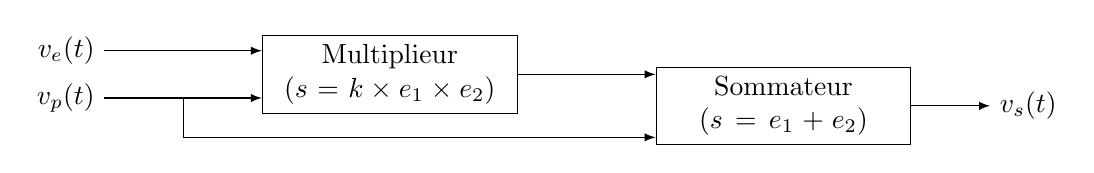
\begin{tikzpicture}
    \node[draw,text width=3cm, text centered] (M) at (0,0) {Multiplieur\\($s=k\times e_1\times e_2$)};
    \node[draw,text width=3cm, text centered] (S) at (5,-0.4) {Sommateur\\($s=e_1+e_2$)};
    \draw (S.west) ++ (0,0.4) coordinate (se1);
    \draw (S.west) ++ (0,-0.4) coordinate (se2);
    \draw[<-,>=latex] (M.west) ++ (0,0.3) --++ (-2,0) node[left] {$v_e(t)$};
    \draw[<-,>=latex] (M.west) ++ (0,-0.3) --++ (-2,0) node[left] {$v_p(t)$};
    \draw[->,>=latex] (M.east) -- (se1);
    \draw[->,>=latex] (M.west) ++ (-1,-0.3) |- (se2);
    \draw[->,>=latex] (S.east) --++ (1,0) node[right] {$v_s(t)$};
  \end{tikzpicture}
\end{center}
Pour démoduler correctement le signal, il ne faut pas que son enveloppe s'annule.}

\begin{enumerate}
  \setcounter{enumi}{2}
  \question{Exprimer $v_s(t)$ en fonction de $v_e(t)$ et $v_{p}(t)$.}
  \question{Dans le cas où $v_{e}(t)$ est sinusoïdal ($v_{e}(t)=A_{e}\cos(2\pi f_{e}t)$), quelle valeur faut-il choisir pour $k$ ?}
    [Tracer l'allure signal modulé en fonction du temps.]
    [Que valent le maximum et le minimum de l'enveloppe du signal modulé.]
  \question{Toujours pour $v_{e}$ sinusoïdal, tracer le spectre du signal modulé $v_{s}(t)$ dans ce cas particulier.}
    [Linéariser l'expression de $v_{s}(t)$. Chaque terme de la somme correspond à un "pic" sur le spectre.]
   \question{On suppose maintenant que $v_e(t)$ est un signal audio. Tracer un spectre possible de $v_e$. Tracer alors le spectre de $v_s$ en prenant $f_p=\SI{520}{kHz}$.}
  \question{Les ondes moyennes s'étendent de $\SI{520}{kHz}$ à $\SI{1620}{kHz}$. Combien de canaux audios peuvent être émis sur cette bande.}
    [À partir de la question précédente, quel "espace" prend un canal ?]
\end{enumerate}

\exercice{Summing amplifier}
\enonce{In the previous exercice, we have seen the necessity for a summing system in order to réalise an amplitude modulation. This system can be realized by the following assembly.
\begin{center}
  \begin{circuitikz}
    \draw (0,0) node[en amp] (ALI) {};
    \draw (ALI.+) --++ (0,-0.7) node[ground] {};
    \draw (ALI.-) --++ (0,1.5) to[R=$R$] ++ (2.3,0) -| (ALI.out) --++ (0.5,0) node[right] {$v_s$};
    \draw (ALI.-) --++ (-1,0) to[R,l_=$R_1$] ++ (-2,0) node[left] {$v_2$};
    \draw (ALI.-) -|++ (-1,1.5) to[R,l_=$R_2$] ++ (-2,0) node[left] {$v_1$};
  \end{circuitikz}
\end{center}}

\begin{enumerate}
  \question{Ascertain the expression of $V_{-}$ as a function of $v_1$ and $v_2$ and $v_s$.}
    [Utiliser la loi des nœuds en termes de potentiels à l'entrée inverseuse de l'ALI.]
    [Écrire la loi des nœuds à l'entrée de l'ALI. Remplacer chacun des courants par son expression à partir de la loi d'Ohm.]
    [Quelle différence de potentiel y a-t-il aux bornes de chaque résistor (en fonction de $v_1$, $v_2$, $v_s$ et $V_{-}$) ?]
  \question{Deduce an expression of $v_s$ as a function of $v_1$ and $v_2$.}
    [Que peut-on dire de $V_{-}$ ?]
    [Le montage est-il stable ou instable ?]
    [Que vaut l'entrée différentielle de l'ALI ?]
  \question{Under which condition does $v_s=-(v_1+v_2)$.}
  \question{The aim is to have ${v_s}_2=v_1+v_2$. Which transfer function needs to be placed after the previous system to obtain ${v_s}_2$ ? Suggest an electronic assembly that would have this transfer function.}
    [Parmi les montages vus, lequel a une fonction de transfert indépendante de $j\omega$ et négative ?]
    [La fonction de transfert d'un amplificateur inverseur est $\underline{H}(j\omega)=-\frac{R_2}{R_1}$.]
\end{enumerate}

\exercice{Démodulation synchrone}
\enonce{
On souhaite démoduler un signal modulé en amplitude $s_{AM}(t)$ avec une porteuse $s_p(t)$ de fréquence $\SI{200}{kHz}$. Le spectre du signal original s'étend entre $0$ et $\SI{10}{kHz}$. On utilise pour cela le montage suivant.
\begin{center}
  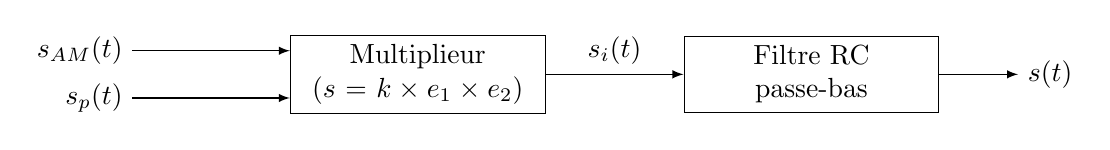
\begin{tikzpicture}
    \node[draw,text width=3cm, text centered] (M) at (0,0) {Multiplieur\\($s=k\times e_1\times e_2$)};
    \node[draw,text width=3cm, text centered] (S) at (5,0) {Filtre RC\\passe-bas};
    \draw[<-,>=latex] (M.west) ++ (0,0.3) --++ (-2,0) node[left] {$s_{AM}(t)$};
    \draw[<-,>=latex] (M.west) ++ (0,-0.3) --++ (-2,0) node[left] {$s_p(t)$};
    \draw[->,>=latex] (S.east) --++ (1,0) node[right] {$s(t)$};
    \draw[->,>=latex] (M.east) -- (S.west) node[midway,above] {$s_i(t)$};
  \end{tikzpicture}
\end{center}}

\begin{enumerate}
  \question{Représenter qualitativement les spectres de $s_{AM}(t)$, $s_p(t)$, $s_i(t)$ et $s(t)$.}
  \question{Proposer des valeurs réalistes pour $R$ et $C$ afin que le signal démodulé $s(t)$ s'approche convenablement du signal modulant.}
    [Dans quelles plages de fréquence peut-on choisir $R$ et $C$ en TP ?]
    [Quelles relations (supérieur, inférieur, très petit devant ou très grand devant) doit vérifier la fréquence de coupure du filtre passe-bas ?]
\end{enumerate}

\exercice{Démodulation par détection d'enveloppe}
\enonce{
On souhaite démoduler un signal modulé en amplitude $e(t)=A_0[1+m\cos(2\pi f_st)]\cos(2\pi f_pt)$. On utilise pour cela le montage ci-dessous appelé détecteur d'enveloppe.
\begin{center}
  \begin{circuitikz}
    \draw (0,0) to[D,i>^=$i$] (2,0) to[R=$R$] (2,-2);
    \draw (2,0) -- (3.5,0) to[C=$C$] (3.5,-2) -- (0,-2);
    \draw[<-,>=latex] (0,-0.1) -- (0,-1.9) node[midway,left] {$e(t)$};
    \draw[<-,>=latex] (4.7,0) -- (4.7,-2) node[midway,right] {$s(t)$};
  \end{circuitikz}
\end{center}}

\begin{enumerate}
  \question{Montrer que lorsque la diode est passante (i.e. qu'elle se comporte comme un fil) $s(t)=e(t)$.}
    [Redessiner le schéma en remplaçant la diode par un fil.]
    [Quelle est la différence de potentiel aux bornes d'un fil ?]
  \question{Déterminer l'équation différentielle vérifiée sur $s(t)$ lorsque la diode est bloquée (i.e. qu'elle se comporte comme un interrupteur ouvert).}
    [Redessiner le schéma en remplaçant la diode par un interrupteur ouvert.]
    [Introduire le courant passant dans le circuit.]
    [En utilisant la relation entre tension et courant pour un condensateur et la loi d'Ohm, obtenir l'équation différentielle demandée.]
  \question{On utilise Python pour simuler l'évolution de $s(t)$ pour deux signaux de taux de modulation différents. Se rendre sur Capytale (code \texttt{0b1c-7216837}) et compléter le code.}
  \question{Lequel des deux signaux sera correctement démodulé ?}
\end{enumerate}

\exercice{Taux de modulation}
La figure ci-dessous représente un signal modulé en amplitude, dont le signal modulant est sinusoïdal.
\begin{enumerate}
  \question{Quelle est la fréquence de la porteuse ?}
  \question{Quelle est la fréquence du signal modulant ?}
  \question{Mesurer le taux de modulation.}
    [Quelles sont les valeurs maximale et minimale de la modulante ?]
    [Comment les valeurs extrémales de la modulante sont reliées au taux de modulation ?]
\end{enumerate}
  \begin{center}
    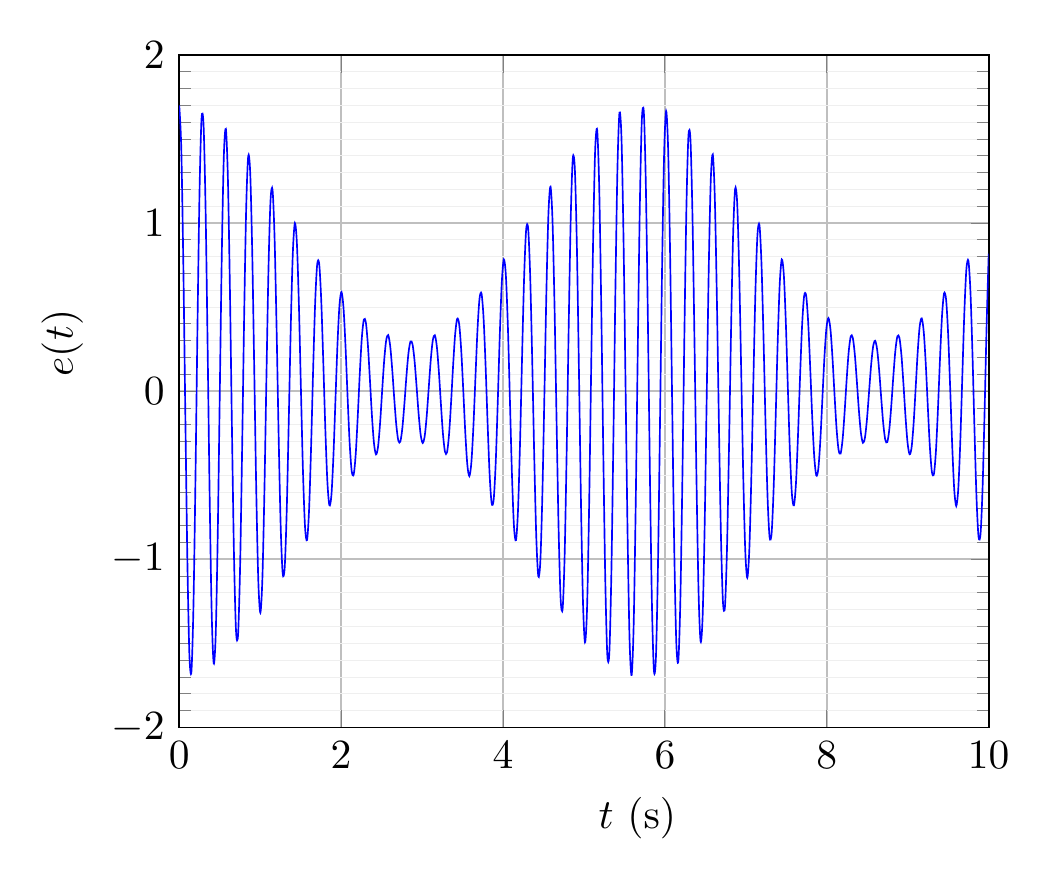
\begin{tikzpicture}[scale=1.5]
      \begin{axis}[
          ymin=-2, ymax=2,
          xmin=0, xmax=10,
          %enlargelimits=true,
          xlabel={$t$ (s)},
          xlabel style={below right},
          ylabel={$e(t)$},
          ylabel style={above right},
          %label style = {at={(ticklabel cs:1.1)}}
          grid=both,
          minor grid style={very thin, lightgray!25}, 
          major grid style={thin},
          minor y tick num=9,
        ]
        \addplot expression[samples=400,domain=0:10, mark=none, smooth] {cos(2*pi*200*x)*(1+0.7*cos(2*pi*10*x))};
      \end{axis}
    \end{tikzpicture}
  \end{center}

\exercice{Thérémine}

  \begin{wrapfigure}{r}{8cm}
    \centering
    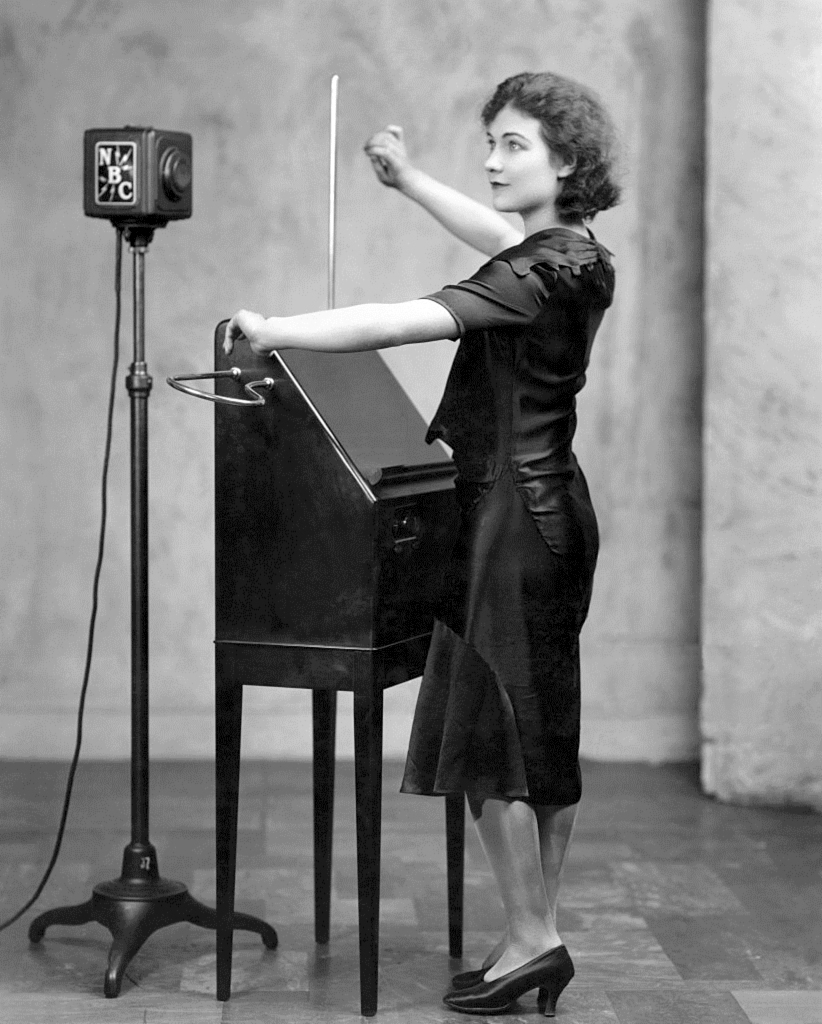
\includegraphics[width=7cm]{images/theremin.jpg}
  \end{wrapfigure}

  On s'intéresse à un Thérémine constitué de deux oscillateurs à relaxation de périodes d'oscillation $T_1=4\frac{R_a}{R_b}RC_1$ et $T_2=4\frac{R_a}{R_b}RC_2$. Le condensateur $C_2$ est constitué d'un condensateur identique à $C_1$ en parallèle d'un condensateur $C'$, lui-même constitué de la main et de l'antenne et variant entre $0$ et $\SI{10}{pF}$.

  Les signaux issus des deux oscillateurs sont envoyés dans un multiplieur dont on note $s(t)$ la sortie.

  \begin{enumerate}
    \question{Exprimer $C_2$ en fonction de $C_1$ et $C'$.}
      [Faire un schéma des deux condensateurs en parallèle.]
      [Écrire la loi des nœuds puis la relation tension-courant pour $C_1$ et $C'$.]
    \question{En supposant $C'\ll C_1$, quelle est la fréquence la plus petite contenue dans le spectre de $s$ ? Elle sera exprimée en fonction de $R_a$, $R_b$, $R$, $C_1$ et $C'$.}
      [Compte tenu de l’approximation, que peut-on dire des fréquences $\frac{1}{T_1}$ et $\frac{1}{T_2}$ ?]
      [Représenter les spectres des tensions de sortie des deux oscillateurs.]
    \question{Quel montage faut-il placer après $s$ pour isoler cette fréquence ? On notera $s'(t)$ la sortie de ce filtre.}
      [Quel filtre laisse passer les basses fréquence et coupe les hautes fréquences ?]
      [Comment peut-on réaliser ce montage avec un condensateur et un résistor ?]
    \question{Quelle valeur doit avoir $C_1$ pour que la fréquence du signal en sortie varie entre $0$ et $\SI{2}{kHz} ?$}
  \end{enumerate}

  \textit{Données : } $R_1=\SI{1}{k\ohm}$ ; $R_2=\SI{2}{k\ohm}$ ; $R=\SI{100}{k\ohm}$ ; $C'\in [0,\SI{10}{pF}]$

\exercice{J'explique à ma grand-mère}
  \textit{Le but de cet exercice est de vous faire expliquer un concept/phénomène avec des mots simples et courants (pas de vocabulaire technique ou scientifique) à une personne de votre entourage. Tachez de faire simple et court, utilisez des analogies avec des choses connues. Vous pouvez vous inspirer de \href{https://www.youtube.com/@MT180_fr}{Ma thèse en 180 secondes}. Profitez-en pour prendre des nouvelles !}

  \begin{enumerate}
    \question{Comment peut-on diffuser plein de stations de radio sur les ondes sans qu'elles se mélangent et comment fait mon poste de radio pour sélectionner celle que je veux écouter ?}
  \end{enumerate}

  % RAJOUTER FM